\chapter{Theory, Current State}
\label{ch:theory}

% TODO
%% What is this chapter about
In this chapter, we will lay down the base for the following text, with the main focus on the Rego language and SMT solving.
Since both topics are under constant development, we will include the possible limitations implied by both technologies.

\section{Open Policy Agent}
\label{sec:opa}

Open Policy Agent (OPA) is a general-purpose policy engine designed to decouple policy decision making from application logic.
Policy decision making refers to the evaluation of conditions that determine whether actions such as access requests, configuration changes, or deployment operations should be permitted or denied.
OPA provides a high-level declarative language and evaluation framework that allows policies to be expressed independently of the systems that enforce them.
OPA can be integrated with diverse systems including microservices, API gateways, Kubernetes admission controls, and CI/CD pipelines.

\begin{figure}
    \label{fig:opa-query-graph}
    \centering
    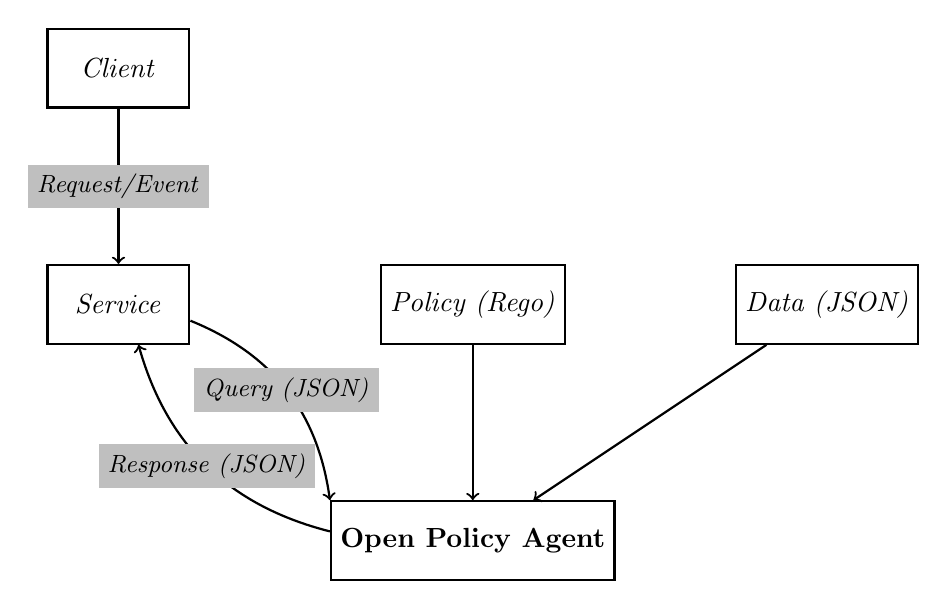
\begin{tikzpicture}[
        s/.style={draw,thick,rectangle,minimum height=10mm, minimum width=18mm},
        e/.style={fill=gray!50},
        xsh/.style={xshift=15mm}
    ]

    \tikzset{
        node distance=30mm,
    }

    \node[s] (client) {\textit{Client}};
    \node[s,below of=client] (service) {\textit{Service}};
    \node[s,right of=service,xsh] (policy) {\textit{Policy (Rego)}};
    \node[s,right of=policy,xsh] (data) {\textit{Data (JSON)}};
    \node[s,below of=policy] (OPA) {\textbf{Open Policy Agent}};

    \draw[->,thick]
        (client) edge node[e] {\small \textit{Request/Event}} (service)
        (service) edge[bend left] node[e] {\small \textit{Query (JSON)}} (OPA.north west)
        (OPA) edge[bend left] node[e] {\small \textit{Response (JSON)}} (service)
        (policy) edge (OPA)
        (data) edge (OPA)
        ;
    
\end{tikzpicture}

    \caption{Structure of communication between a service and OPA.}
\end{figure}

The motivation for adopting OPA arises from the need to manage and enforce policies consistently across heterogeneous environments.
Traditional approaches often embed policy logic directly into application code, leading to duplicated logic, inconsistencies, and challenges in governance and auditing.
Policy as code is the paradigm of expressing access control, security, compliance, and other governance policies in a machine-readable, executable form.
It elevates policy definitions to first-class artifacts in version control systems, enabling automated testing, review, and lifecycle management similarly to application code.
OPA embodies this paradigm by treating policies as modular, executable artifacts written in a dedicated language.

The core language used by OPA for policy expression is \emph{Rego}.
Rego is a purpose-built declarative policy language inspired by Datalog, designed to reason over structured documents, most significantly in JSON format.
Rego allows authors to express queries, rules, constraints, and derived values without specifying a procedural control flow.
Because Rego is declarative, users define what constitutes a valid decision rather than how to compute it; under the hood, OPA’s evaluation engine determines an efficient execution plan for query evaluation.
Rego’s declarative nature enables optimized evaluation and composability of policy rules.

Figure \ref{fig:opa-query-graph} depicts the high-level point of view on the communication between a service and OPA.
Client requests are transformed into queries to the OPA; we will often call these queries \emph{input} in the following text.
The OPA then evaluates the query with respect to a policy specified in Rego and a JSON document representing the service data (e.g., list of permitted servers).

Rego policies are composed in \emph{modules}.
A module consists of exactly one package declaration, zero or more import statements, and zero or more rule definitions.
The package declaration defines a namespace for rules, enabling modularization and reuse across policy sets.
Import statements allow references to external data or built-in functions.
Rules constitute the core logical expressions that define policy outcomes.
Each rule has a \emph{head} and a \emph{body}; the head names the rule and optionally declares keys and values, while the body contains logical expressions that must be satisfied for the rule to apply.
A rule in Rego can be either \emph{complete} or \emph{partial}.
A complete rule assigns a specific value to a variable when its body conditions are true.
A partial rule may define part of a set or object document by generating entries that satisfy the body expressions.
Variables in Rego are implicitly existentially quantified; the evaluation finds bindings that satisfy all expressions in the rule body.
Universal quantification constructs such as every provide an explicit mechanism to express conditions over entire collections.

Every rule is composed of the \texttt{head} (an assignment) and the \texttt{body}, which is a set of expressions, that are all evaluated as a \texttt{boolean} value.
If all of the expressions in the rule body hold, i.e., their conjunction is evaluated as \texttt{true}, the assignment in the rule head is also valid.
Otherwise, the assignment is not executed.
It is therefore mandatory, that only one rule body can be true for a variable.

\paragraph{Example.}
Let \texttt{a := 1 if \{ b == "valid" \}} be a rule in Rego policy $\mathcal{R}$.
Then \texttt{a := 1} is the rule head and \texttt{\{ b == "valid" \}} is the rule body, containing a single expression.
When $b$ is equal to \texttt{"valid"}, then \texttt{a} is equal to $1$.

There are special rules, called the defaults, in the form \texttt{default <head>}, meaning they are missing a body and the \texttt{<head>} represents an assignment into variable $v$.
If for all rules about $v$, none have a body that evaluates to \texttt{true}, its assignment from the default rule applicated.
In the case, that even the default rule is missing and every body evaluates to \texttt{false}, the variable is \texttt{undefined}.


Rules operate on documents—hierarchical structured data typically represented as JSON.
When OPA evaluates a policy, it accepts an input document (representing the context for a decision) along with arbitrary structured base data; policies then generate decision outputs that may be booleans, messages, sets, or arbitrarily complex data.
In practice, the input to OPA might include user identity, resource attributes, and environmental context, while data documents might include role definitions, access control lists, or trusted configuration parameters.
The output of policy evaluation is returned to the calling system, which can then enforce the decision.

As we can see in Figure \ref{fig:opa-input-example} the input is in the JSON format, as one document.
Moreover, it is just a single object, which can be queried with the rules specified in Rego Policy Language.

Rego supports composite types including arrays, objects, and sets.
These types enable succinct expressions over nested data structures.
For example, rules can join elements of collections implicitly, bind variables to specific parts of the input, or generate sets of conditionally derived values.
Built-in functions provide common operations such as string manipulation, arithmetic, aggregation, and type inspection; these can be called within rule bodies to facilitate complex logic.

Because policies are declarative, authors are freed from specifying how rule evaluation proceeds.
Instead they express logical conditions that describe acceptable or unacceptable states.
This declarative nature simplifies reasoning about policy correctness and supports automated tooling to optimize, test, and validate policy sets.
Furthermore, because Rego is domain-agnostic, policies can describe decisions that extend beyond simple allow/deny semantics to produce structured decision outputs tailored to the needs of diverse enforcement points.

\begin{figure}
    \label{fig:opa-input-example}
    \centering
    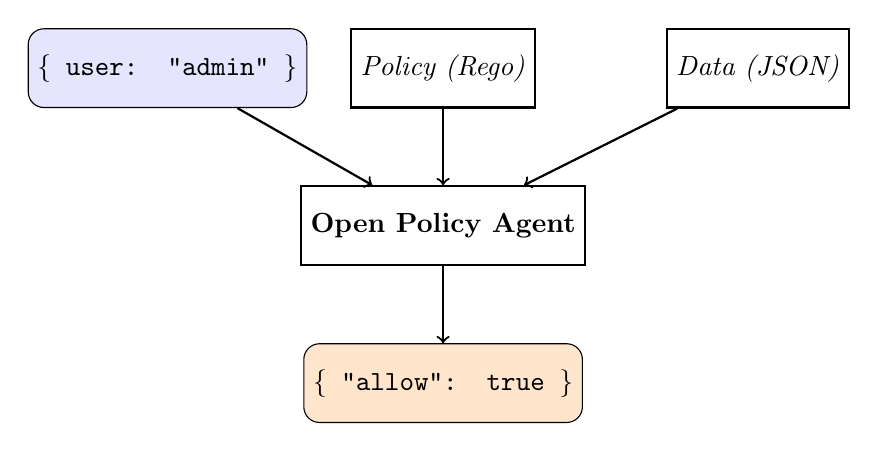
\begin{tikzpicture}[
    s/.style={draw,thick,rectangle,minimum height=10mm, minimum width=18mm},
    e/.style={fill=gray!50},
    code/.style={draw,fill=blue!10,rectangle,minimum height=10mm, minimum width=18mm,rounded corners=2mm},
    xsh/.style={xshift=15mm},
]

    \tikzset{
        node distance=20mm,
    }

    \node[code] (input) {\texttt{\{ user: "admin" \}}};
    \node[s,right of=input,xshift=15mm] (policy) {\textit{Policy (Rego)}};
    \node[s,right of=policy,xshift=20mm] (data) {\textit{Data (JSON)}};
    \node[s,below of=policy] (OPA) {\textbf{Open Policy Agent}};
    \node[code,fill=orange!20,below of=OPA] (output) {\texttt{\{ "allow": true \}}};

    \draw[->,thick]
        (input) edge (OPA)
        (policy) edge (OPA)
        (data) edge (OPA)
        (OPA) edge (output)
    ;

\end{tikzpicture}

    \caption{Example of input and output of Open Policy Agent.}
\end{figure}

\section{SMT Solving}
\label{sec:smt}

% TODO
%% What is complete, sound, ...
% Inference rules
% Array theory
% Unint func theory

This section will describe the details behind SMT which the work of this thesis is laid upon.
This involves looking at the basic functionality of SMT and a quick dive into the inner workings that imply the possible limitations.
In adition, I will describe the \ziii SMT solver which is used in the implementation of this work to evaluate the SMT-LIB formulae.
Since this solver allows reasoning over theories, which are not explicitly in the SMTLIB2 standart and which are essential to this work, they will also be discussed.

\subsection{Preliminaries}

\paragraph{SAT Solving.}
% Propositional formula ...
% A literal $l$ is either a variable $x_i$ or its complement $\neg x_i$.
% A clause $\omega$ is a disjunction of literals.
% Let formula
Propositional formulas are represented in Conjunctive Normal Form (CNF).
A CNF formula is represented using $n$ boolean variables $x_1, x_2, \dots , x_n$ and a boolean assignment $\mathcal{A}$ maps varaibles $x_i$ to truth values 0 (\texttt{false}) or 1 (\texttt{true}) for $0 \leq i \leq n$.
A literal $l$ is either a variable $x_i$ (i.e., a positive literal) or its complement $\neg x_i$ (i.e., a negative literal).
A clause $\omega$ is a disjunction of literals and a CNF formula $\phi$ is a conjunction of clauses.
For a boolean assignment $\mathcal{A}$, $\omega$ is \emph{satisfied} if at least one of its literals is mapped to \texttt{true} and $\phi$ is satisfied if all its clauses are satisfied.
In such case, we say that $\mathcal{A}$ is \emph{solution} to $\phi$.
A formula is \emph{satisfiable} (\emph{SAT}) if there exists at least one solution to it, and \emph{unsatisfiable} (\emph{UNSAT}) otherwise.
Finding such solution is called the \emph{Boolean Satisfiability problem} and it is traditionally referred to as the \emph{SAT problem}.

\begin{example}
    Consider the following formula $\phi = (x_1 \lor x_2 \lor \neg x_3) \land (x_2 \lor x_3) \land(\neg x_1 \lor \neg x_2 \lor \neg x_3)$.
    This formula has 3 variables, 3 clauses, and is satisfiable under the assignment $x_1 \rightarrow 1, x_2 \rightarrow 1, x_3 \rightarrow 0$.
\end{example}

%% TODO completeness, decidability

\paragraph{Satisfiability Modulo Theories.}
The defining problem of Satisfiability Modulo Theories (SMT) is checking whether a given (closed) logical formula $\phi$ is satisfiable, not in general but in the context of some background theory $\T$ which constrains the interpretation of the symbols used in $\phi$.
Technically, the SMT problem for $\phi$ and $\T$ is the question of whether there is a model of $\mathcal{T}$ that makes $\phi$ true.
\emph{SMT solver} is a software that implements a procedure for satisfiability modulo some given theory. 





%% SMT-LIB, theories, soundness, completeness
\subsection{SMT-LIB}

Satisfiability Modulo Theories is an area of automated deduction that studies methods for checking the satisfiability of first-order formulas with respect to some logical theory $\mathcal{T}$ of interest. \cite{smt:sm-theories, smt:first-ord-logic}
What sets apart SMT from general automated deduction is that the background theory $\mathcal{T}$ need not be finitely or even first-order axiomatizable, and that specialized inference methods are used for each theory.
By being theory-specific and restricting their language to certain classes of formulas (such as, typically but not exclusively, quantifier-free formulas), these specialized methods can be implemented in solvers that are more efficient in practice than general-purpose theorem provers.

The SMT-LIB Standard is an international initiative and specification that defines a common language and infrastructure for interacting with SMT solvers.
SMT-LIB aims to facilitate research, development, comparison, and benchmarking of SMT solvers by providing rigorous definitions of languages, theories, and interfaces used in the automated reasoning community.
The initiative also supports a large library of benchmark problems written in a standardized format.

The SMT-LIB Standard Version defines a formal language for writing logical formulas, specifying background theories, defining logics, and interacting with SMT solvers via a command-based interface. The standard’s objectives include: providing a common input/output language for SMT solvers; defining a standard set of sorts, functions, and predicates for background theories; and supporting structured benchmark libraries for experimental evaluation.

SMT-LIB’s language is based on many-sorted (typed) first-order logic with equality, where terms and formulas are strongly typed and structured according to defined sorts such as Bool, Int, and user-defined or theory-specific sorts.
Scripts in the SMT-LIB language consist of commands that declare symbols, assert formulas, query solver actions (e.g., \texttt{check-sat}), and interact with solver responses.
SMT-LIB’s syntax uses S-expressions similar to Lisp to represent terms and commands.

The standard separates concerns into clearly defined components:
\begin{itemize}
    \item \emph{Formula language} — a typed logical language for defining SMT problems.
    \item \emph{Theory declarations} — definitions of sorts and function symbols that form the semantic basis for logical theories (e.g., integers, arrays, bit vectors, strings).
    \item \emph{Logic specifications} — combinations of theory signatures and syntactic restrictions that define classes of admissible formulas.
    \item \emph{Command language} — a textual interface for communicating with SMT solvers, including declaring symbols, asserting constraints, checking satisfiability, and retrieving models.
\end{itemize}

The standard also maintains a catalog of benchmark problems in the SMT-LIB format, grouped by logics and used in community-driven evaluations such as SMT-COMP.
These benchmarks support the systematic assessment of solver performance and feature diverse problem classes across background theories.

The SMT-LIB standard distinguishes between \emph{basic} theories and \emph{combined} theories.
Basic theories, such as the theory of real numbers, the theory of arrays, the theory of fixed-size bit vectors and so on, are those explicitly defined in the SMT-LIB catalog.\footnote{The catalog of basic theories in SMT-LIB is avaliable at \url{https://smt-lib.org}.}
Combined theories are defined implicitly in terms of basic theories by means of a general modular combination operator.
The difference between a basic theory and a combined one in SMT-LIB is essentially operational.
Some SMT-LIB theories, such as the theory of finite sets with a cardinality operator, are defined as basic theories, even if they are in fact a combination of smaller theories, because they cannot be obtained by modular combination.

%% TODO quantifiers

\subsection{Z3}

\textit{The information about \ziii is taken from \cite{z3} and \cite{z3:web}.}

\ziii is SMT solver from Microsoft Research with its first external release dating back to 2007.
Its main purpose is solving problems that arise in software verification and analysis.
\ziii integrates support for a variety of theories, with the most prevalent for this work being linear integer arithmetic, strings, and arrays.

\ziii is implemented in C++ and it is designed to be highly extensible, thanks to its
modularity. From a high-level point of view, \ziii integrates:
\begin{itemize}
    \item 
        \emph{Core theory SAT solver.} Davis–Putnam–Logemann–Loveland (DPLL) algorithm based solver of propositional logic. 
        This solver is used to handle equalities and uninterpreted functions.
    \item 
        \emph{Satellite solvers.}
        Specialized theory solvers.
    \item 
        \emph{E-matching abstract machine.}
        This component finds instantiations of quantified formulas that lead to a satisfiable solution.
\end{itemize}

\begin{figure}
    \label{fig:z3-system-arch}
    \centering
    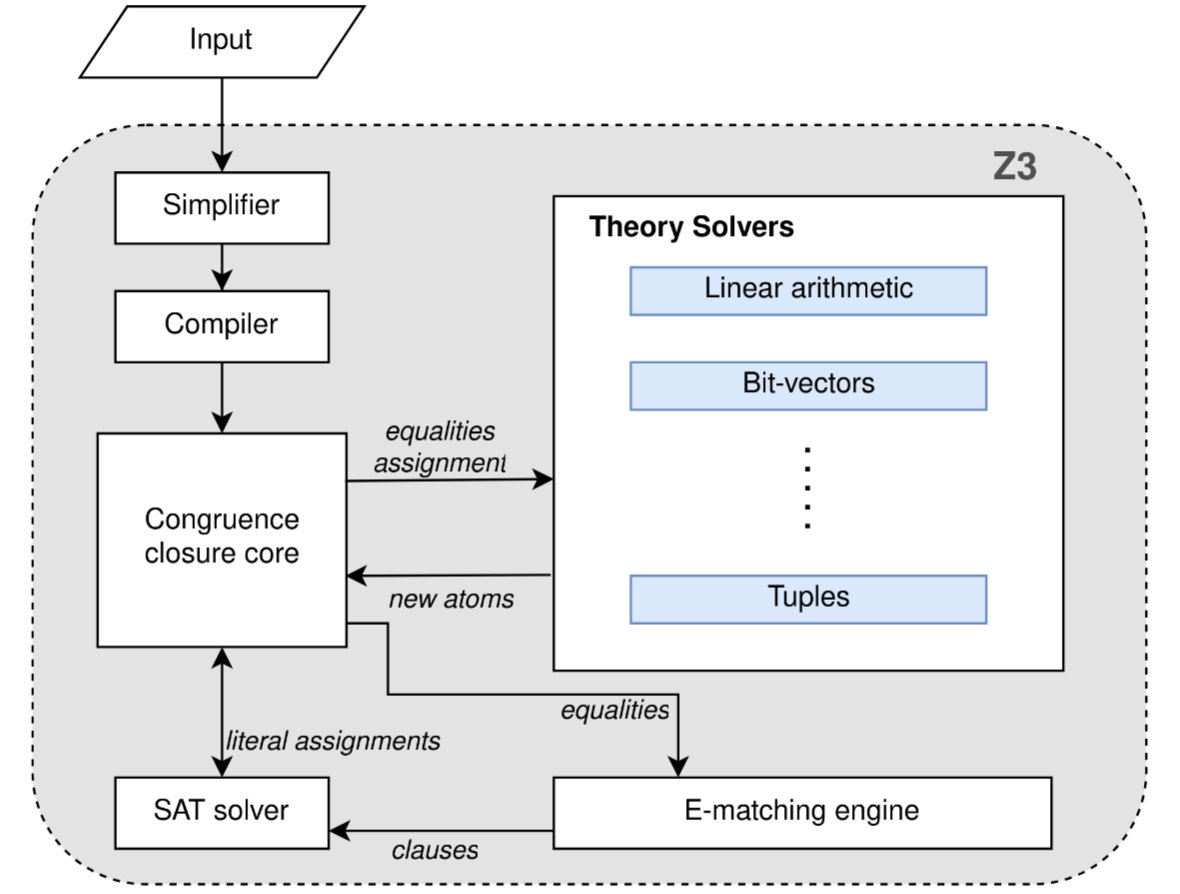
\includegraphics[width=0.75\textwidth]{figures/z3-system-arch.png}
    \caption{System architecture of Z3.}
\end{figure}

A schematic overview of the structure of \ziii is shown in Figure~\ref{fig:z3-system-arch}.
Essential components of \ziii are then described as follows:

\paragraph{Input.}
It is possible to interact with \ziii using either a textual format or a binary API.
As mentioned in \cite{z3:web} the textual input can appear in several different forms with the most notable one being SMTLIB2 format, which uses a LISP-like syntax.
Programmatic interaction with this tool is possible through an API from Python, C, C++, Go, Java, and other languages.

\paragraph{Simplifier.}
To offer the maximal performance, input formulas are first simplified in an incomplete, but efficient process.
The simplify a formula, this component applies standard algebraic reduction rules.
For example $p \land true$ can be reduced to just $p$.
In this process, the simplifier even tries to identify equational definitions (such as $x = 4$) within a context and using given definition, it then reduces the remaining formula.
For example, $x = 4 \land q(x)$ can be this way reduced to $x = 4 \land q(4)$.

\paragraph{Compiler.}
This component takes a simplified abstract syntax tree representation of the input formula and converts it into a different data structure.
Such data structure comprises a set of clauses and congruence-closure nodes.

\paragraph{Atoms.}
Atoms, or atomic formulas, are formulas, which cannot be further decomposed into simpler logical components.
Atoms can be either equalities or theory specific atoms (for instance an arithmetical inequality).

\paragraph{Congruence Closure Core.}
The congruence closure core receives truth assignments to atoms from the SAT solver.
Such asserted equalities are then propagated using a data structure called E-graph, with nodes in such a graph pointing to one or more theory solvers.
A merge of two nodes is propagated to all theory solvers pointed to by the given nodes.
The core also propagates the effects of the theory solvers.
Such effects can range over inferred equalities to assignment of atoms to true or false.
In the case of non-convex theories (i. e., theories for which quantifier elimination and other automated reasonings are complicated or impossible), the theory solvers can also produce fresh atoms.

\paragraph{Theory Solvers.}
\ziii’s ability to solve constraints of a specific theory comes from its integration with a solver for given theory.
These specialized solvers are called theory solvers or satellite solvers.
As shown in the Figure TODO, solvers are used to produce new atoms for given assignment from the \ziii core, i.e., the congruence closure core.

\paragraph{E-matching Engine.}
This engine is used reasoning over quantifiers, where \ziii combines a well known approach with new algorithms described in [17].
In this process, it operates over the E-graph data structures and passes generated clauses to the SAT solver.

\paragraph{SAT Solver.}
\ziii leverages the power of state-of-the-art SAT solver which integrates standard search pruning methods.
It is used to control boolean case splits generated by the \ziii core (sometimes with the extra step of E-matching).

\gap

The components of \ziii offer a special set of tools and techniques which help the SMT
solver stand out amongst others. The most significant being:

\paragraph{Deleting Clauses.}
During quantifier instantiation, clauses containing new atoms are as a side-effect produced into the search space.
When such clause is useless in closing branches, it is garbage collected together with its atoms and terms.
Conflict clauses are not deleted, but retained as a side-effect.

\paragraph{Relevancy Propagation.}
In practice, several atoms appearing in a goal of an SMT solver are irrelevant, or so called \emph{don’t cares}.
For expensive theories, \ziii ignores such atoms and inference rules.
To distinguish relevant atoms from don’t cares, \ziii uses algorithm described in TODO.

\paragraph{Model Generation.}
\ziii has the ability to produce models as part of the output.
Such models assign values to the constants in the input and generate partial function graphs for predicates and function symbols.

\gap

\ziii has estabilished itself as a state-of-the-art SMT solver since its release in 2007.
It has remained with this title to this day, because of his stability, efficiency and modularity.
It also supports a variety of non-standart theories, such as Array theory.
For these reasons, we have decided to focus the SMT code generation presented in the next chapters onto it.

\section{Arrays in Z3}

\textit{Information provided in this section is based on the research from \cite{z3:array-theory}.}

Arrays constitute one of the fundamental interpreted theories provided by Z3.
They are used to model finite or infinite memory structures, such as program heaps, buffers, or lookup tables, in a mathematically precise yet flexible way.
This section summarizes the basic concepts of the theory of arrays as used in Z3, following the standard presentation adopted in SMT-based verification.

An array is viewed as a total function from an index sort to an element sort.
For given sorts $I$ (indices) and $E$ (elements), the array sort is denoted by $\text{Array}(I, E)$.
Intuitively, an array assigns to every index $i \in I$ a value $e \in E$.
Arrays in Z3 are immutable objects; operations on arrays therefore return new arrays rather than modifying existing ones.

\subsection{Read and Store Operations}

The behavior of arrays is characterized by two primary operations: \emph{read} and \emph{store}. The read operation, usually written as
$$
\text{select}(a, i),
$$
returns the element stored in array $a$ at index $i$.
Semantically, this corresponds to function application.

The store operation,
$$
\text{store}(a, i, v),
$$
produces a new array that is identical to $a$ at all indices except possibly at $i$, where it yields the value $v$.
The original array $a$ remains unchanged.
This functional view is essential for reasoning in first-order logic and enables equational reasoning about array updates.

The interaction between read and store is governed by two fundamental axioms.
First, reading from the index that was just updated returns the stored value:
$$
\text{select}(\text{store}(a, i, v), i) = v.
$$
Second, reading from a different index is unaffected by the store:
$$
i \neq j ;\Rightarrow; \text{select}(\text{store}(a, i, v), j) = \text{select}(a, j).
$$
Together, these properties precisely capture the intended semantics of array updates.

\subsection{Constant Arrays and the $K$ Operator}

In addition to read and store, Z3 provides a constant array constructor, commonly denoted by the $K$ operator. For a given element value $v \in E$, the term
$$
K(v)
$$
denotes an array that maps every index to $v$.
Constant arrays are useful for modeling uniform initialization, such as freshly allocated memory filled with a default value.

Formally, for all indices $i$, the following property holds:
$$
\text{select}(K(v), i) = v.
$$
Constant arrays can be combined with store operations to describe more complex memory states, for example by starting from a uniform array and applying a sequence of updates.

\subsection{Summary}

The theory of arrays in Z3 is based on a small set of well-defined operations and axioms.
Arrays are total, immutable functions; \texttt{select} models lookup, \texttt{store} models functional update, and the $K$ operator provides uniformly initialized arrays.
Despite their simplicity, these constructs are expressive enough to model a wide range of data structures encountered in program analysis and formal verification.
